\begin{figure}[t]
    \centering
    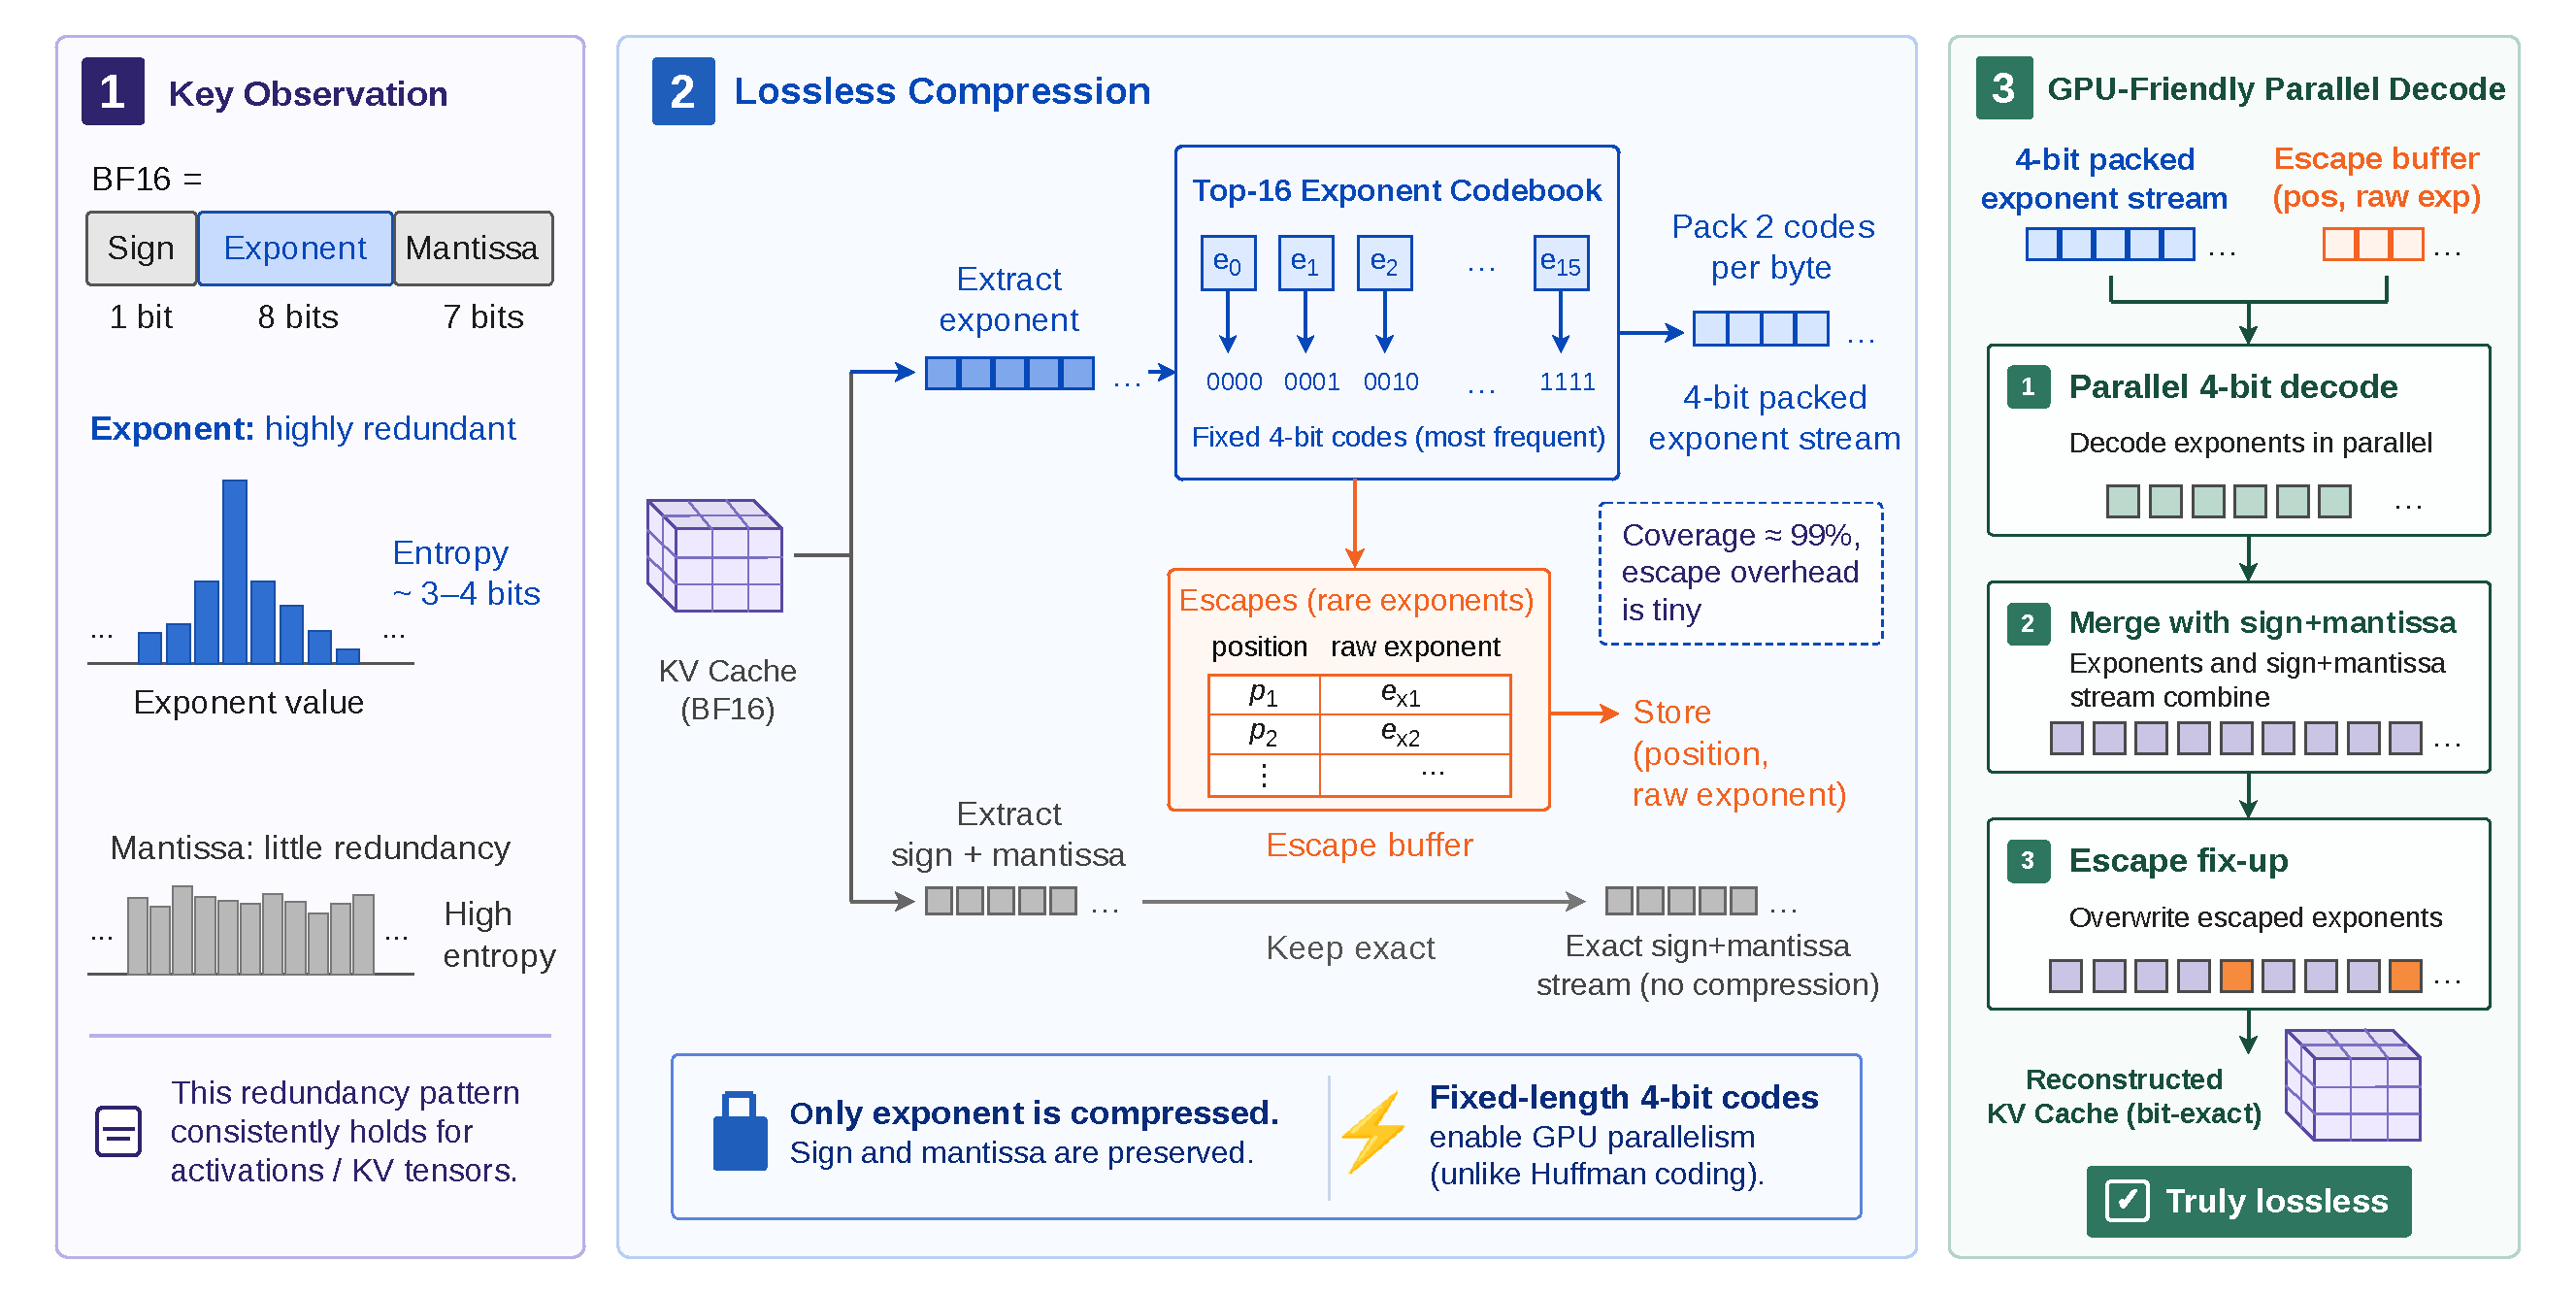
\includegraphics[width=\textwidth]{lossless-paper/figure/main.pdf}
    \caption{\textbf{Overview of SplitZip for lossless KV-cache compression.} SplitZip exploits the redundancy of the BF16 exponent field while keeping sign and mantissa exact. It encodes the most frequent exponent values with fixed 4-bit codes and stores rare values in a small escape buffer with their positions and raw exponents. This design enables GPU-friendly parallel decoding and reconstructs the original KV cache bit-exactly.}
    \label{fig:main}
\end{figure}

\section{\splitzip}
\label{sec:method}

\subsection{Preliminary: Compressing the Exponent}
\label{sec:method_motivation}

Lossless compression of floating-point tensors is highly asymmetric across bit fields. A BF16 value contains one sign bit, eight exponent bits, and seven mantissa bits. Prior work shows that most redundancy lies in the exponent field: DFloat11~\cite{dfloat11} reports that BF16 weight exponents usually have entropy below three bits, while the mantissa is close to incompressible. KV-cache activations follow the same trend, although their wider numerical range increases exponent entropy to roughly three to four bits, as shown in Tab.~\ref{tab:exponent}. This motivates SplitZip to preserve sign and mantissa bits exactly and compress only the exponent field.

Most existing lossless neural-network compression systems target weights, where compression can be performed offline and the main concern is decompression overhead~\cite{dfloat11,zipnn}. In prefill--decode disaggregated serving, however, KV caches are generated, transferred, and consumed online. Both compression and decompression therefore lie on the latency-critical path. SplitZip is designed for this setting: it reduces transferred bytes while keeping both codec directions simple and GPU-friendly.

\subsection{Method}
\label{sec:method_overview}

SplitZip combines fixed-length exponent coding with explicit escape capture, as illustrated in Fig.~\ref{fig:main}. For a BF16 value represented as a 16-bit integer $x_i$, SplitZip extracts

\[
    e_i = (x_i \gg 7) \mathbin{\&} 0xff,
    \qquad
    a_i = ((x_i \gg 8) \mathbin{\&} 0x80) \;|\; (x_i \mathbin{\&} 0x7f),
\]
where $e_i$ is the 8-bit exponent and $a_i$ is the exact sign--mantissa byte.
Given a decoded exponent $\hat e_i$, the original BF16 bit pattern is reconstructed as
\[
    \hat x_i =
    ((a_i \mathbin{\&} 0x80) \ll 8)
    \;|\;
    (\hat e_i \ll 7)
    \;|\;
    (a_i \mathbin{\&} 0x7f).
\]

The sign bit and mantissa bits are stored losslessly as an 8-bit stream. 
For the exponent stream, SplitZip uses a calibrated codebook containing the 16 most frequent exponent values. 
Each common exponent is encoded using a 4-bit code, and two 4-bit codes are packed into one byte. 
Exponent values outside the top-16 set are treated as escape values. 
For each escape value, SplitZip records its element position as a 32-bit integer and its raw exponent value as an 8-bit integer.

Let $\mathcal{C}=\{c_0,\ldots,c_{15}\}$ be the calibrated top-16 exponent set and $\mathcal{E} = \{ i \mid e_i \notin \mathcal{C} \}$ be the escape set. 
For a tensor with $N$ BF16 elements and $M=|\mathcal{E}|$ escaped exponents, SplitZip stores
\[
    B_{\mathrm{SZ}}
    =
    \underbrace{N}_{\text{sign--mantissa}}
    +
    \underbrace{\frac{N}{2}}_{\text{4-bit exponent codes}}
    +
    \underbrace{5M}_{\text{escape positions and values}}
    =
    N\left(\frac{3}{2}+5\epsilon\right)
    \qquad Bytes.
\]
Here the $\epsilon=M/N$ is the escape rate. 
Since the uncompressed BF16 tensor uses $B_{\mathrm{raw}}=2N$ bytes, the compression ratio is
\[
    \rho
    =
    \frac{B_{\mathrm{raw}}}{B_{\mathrm{SZ}}}
    =
    \frac{2}{\frac{3}{2}+5\epsilon}.
\]
When the escape rate is negligible, $\rho$ approaches $4/3$.

The first two terms form the dense, regular compression path, while the final term is a sparse correction stream. 
When the top-16 exponent coverage is high (covers greater than 99\%.), $M$ is very small, so the escape overhead is negligible compared with the reduction from replacing each 8-bit exponent with a 4-bit code.

The encoding path contains two GPU-friendly stages. 
The first stage performs the dense transformation: it extracts the exponent, maps it through the encoding lookup table, packs two 4-bit codes into one byte, and stores the sign--mantissa stream exactly. 
The second stage scans the original exponent stream and compacts all exponents not covered by the top-16 codebook into the escape-position and escape-value arrays. 
Using a separate escape-collection stage keeps the common path simple and regular.

Decoding follows the reverse order. 
SplitZip first unpacks each byte into two 4-bit codes, maps each code through a 16-entry decoding lookup table, and reconstructs a BF16 bit pattern by combining the decoded exponent with the stored sign--mantissa bits. 
Since escaped elements were assigned an arbitrary dummy 4-bit code during dense encoding, they may initially decode to an incorrect common exponent. 
SplitZip then applies the sparse correction stream: for each recorded escape position, it overwrites the reconstructed exponent with the exact raw exponent value. 
This final overwrite makes the overall codec strictly lossless.

The design is intentionally aligned with GPU execution. 
The main encode and decode paths use fixed-width loads, stores, bit shifts, and table lookups. 
The decoding table has only 16 entries, so lookup overhead is small and cache-friendly. 

\subsection{Calibration}
\label{sec:method_calibration}

Computing an exact exponent histogram during every compression call would be expensive, SplitZip performs a one-time calibration step on a small representative dataset. 
During calibration, SplitZip extracts all exponent values from the calibration tensors, counts their frequencies, selects the top-16 exponents, and constructs three lookup tables: an encoding table from raw exponent values to 4-bit codes, a decoding table from 4-bit codes back to raw exponent values, and a membership table for detecting escapes. This calibration-based design removes histogram construction from the online compression path. 

Although the codebook is selected using a calibration dataset, our experiments show that the selected high-frequency exponent set generalizes well across inputs. 

\subsection{Top-16 Instead of Top-15}
\label{sec:method_top16}

A natural alternative to indentification of escape value is to reserve one coded value as an explicit escape token.
This top-15-plus-escape-token design allows the decoder to infer escape positions directly from the packed exponent-code stream, thereby reducing the escape positions overhead. 

However, this design also reduces the number of directly represented common exponents from 16 to 15 and introduces special-case handling into the dense decode path.

SplitZip instead uses all 16 possible 4-bit codes for common exponent values. 
Escaped exponents are assigned a dummy code in the packed stream and are later corrected using the explicit escape-position array. 
It increases codebook coverage by retaining the 16th most frequent exponent and preserves a uniform dense decoding path: every element is decoded by the same 4-bit lookup operation.

The objective is not only to maximize the compression ratio, but also to maximize end-to-end pipeline throughput. 
A codec with marginally smaller metadata can still be slower if it introduces divergence or serialized handling into the common path. 
By using top-16 coding and sparse post-correction, SplitZip keeps the dominant computation simple and parallel.

\subsection{Extension to FP8 KV Caches}
\label{sec:method_fp8}

SplitZip can also be applied to FP8 KV caches by adapting the exponent code width to the FP8 format. 
We consider both E5M2 and E4M3. 
For E5M2, the 5-bit exponent can be compressed with either a 4-bit top-16 code or a 3-bit top-8 code. For E4M3, a 4-bit code would not reduce the exponent size, so SplitZip uses a 3-bit top-8 code.
FP8 offers less redundancy than BF16 because the original representation is already smaller, but the same fixed-code-plus-escape principle still applies.

